%%%%%%%%%%%%%%%%%%%%%%%%%%%%%%%%%%%%%%%%%
% Dreuw & Deselaer's Poster
% LaTeX Template
% Version 1.0 (11/04/13)
%
% Created by:
% Philippe Dreuw and Thomas Deselaers
% http://www-i6.informatik.rwth-aachen.de/~dreuw/latexbeamerposter.php
%
% This template has been downloaded from:
% http://www.LaTeXTemplates.com
%
% License:
% CC BY-NC-SA 3.0 (http://creativecommons.org/licenses/by-nc-sa/3.0/)
%
%%%%%%%%%%%%%%%%%%%%%%%%%%%%%%%%%%%%%%%%%

%----------------------------------------------------------------------------------------
%	PACKAGES AND OTHER DOCUMENT CONFIGURATIONS
%----------------------------------------------------------------------------------------

\documentclass[final,hyperref={pdfpagelabels=false}]{beamer}

\usepackage[orientation=portrait,size=a2,scale=1.4]{beamerposter} % Use the beamerposter package for laying out the poster with a portrait orientation and an a0 paper size

\usetheme{I6pd2} % Use the I6pd2 theme supplied with this template

\usepackage[english]{babel} % English language/hyphenation

\usepackage{amsmath,amsthm,amssymb,latexsym} % For including math equations, theorems, symbols, etc

%\usepackage{times}\usefonttheme{professionalfonts}  % Uncomment to use Times as the main font
%\usefonttheme[onlymath]{serif} % Uncomment to use a Serif font within math environments

\boldmath % Use bold for everything within the math environment

\usepackage{booktabs} % Top and bottom rules for tables

\graphicspath{{figures/}} % Location of the graphics files

\usecaptiontemplate{\small\structure{\insertcaptionname~\insertcaptionnumber: }\insertcaption} % A fix for figure numbering

%----------------------------------------------------------------------------------------
%	TITLE SECTION 
%----------------------------------------------------------------------------------------

\title{\huge HScraper - A Haskell library to parse, crawl and scrape webpages} % Poster title
\author{Ayush Agarwal, Nishant Gupta, M.Arunothia} % Author(s)

\institute{Indian Institute of Technology Kanpur} % Institution(s)

%----------------------------------------------------------------------------------------
%	FOOTER TEXT
%----------------------------------------------------------------------------------------

\newcommand{\leftfoot}{Submitted to Prof. Piyush P Kurur for partial fulfilment of the course requirements for CS653A, IITK} % Left footer text

\newcommand{\rightfoot}{} % Right footer text

%----------------------------------------------------------------------------------------

\begin{document}

\addtobeamertemplate{block end}{}{\vspace*{2ex}} % White space under blocks

\begin{frame}[t] % The whole poster is enclosed in one beamer frame

\begin{columns}[t] % The whole poster consists of two major columns, each of which can be subdivided further with another \begin{columns} block - the [t] argument aligns each column's content to the top

\begin{column}{.02\textwidth}\end{column} % Empty spacer column

\begin{column}{.465\textwidth} % The first column

%----------------------------------------------------------------------------------------
%	OBJECTIVES
%----------------------------------------------------------------------------------------

\begin{block}{Aim}

 The aim of this project is to build a Haskell library that enables the user to correctly parse, crawl and scrape web-pages. 
\end{block}

\begin{block}{Motivation}
 

\end{block}


%----------------------------------------------------------------------------------------
%	INTRODUCTION
%----------------------------------------------------------------------------------------
            
\begin{block}{Introduction}

Inductive Logic Programming has been defined as the intersection of Machine Learning and Logic Programming. The examples given to the learning system are expressed in a logical programming language such as prolog. Moreover, the conceptes which the learning system develops from the examples are also expressed in the same language. This feature of ILP has been used in this project because it enables us to get attribute values well defined in the language of logic only. ~\cite{progol_manual}  

\end{block}

%----------------------------------------------------------------------------------------
%	MATERIALS
%----------------------------------------------------------------------------------------

\begin{block}{Data Base}

\begin{columns} % Subdivide the first main column
\begin{column}{.54\textwidth} % The first subdivided column within the first main column
\begin{itemize}
\item {\large Source} https://archive.ics.uci.edu/ml/machine-learning-databases/chess/king-rook-vs-king/
\item {\large Format}
\begin{itemize}
\item White King file (column)
\item White King rank (row)
\item White Rook file
\item White Rook rank
\item Black King file
\item Black King rank
\item optimal depth-of-win for White in 0 to 16 moves,otherwise draw.
\end{itemize}
\end{itemize}
\end{column}
~\cite{data}
\begin{column}{.43\textwidth} % The second subdivided column within the first main column
\centering
\begin{figure}
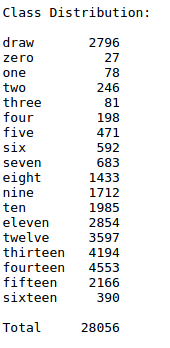
\includegraphics[width=0.5\linewidth]{data_class_distribution.png}
\caption{Distribution of data}
\end{figure}
\end{column}
\end{columns} % End of the subdivision

\end{block}

%----------------------------------------------------------------------------------------
%	METHODS
%----------------------------------------------------------------------------------------

\begin{block}{Method}
\begin{itemize}
\item Progol is an implementation of Inductive Logic Programming used in computer science that combines "Inverse Entailment" with "general-to-specific search" through a refinement graph. "Inverse Entailment" is used with mode declarations to derive the most-specific clause within the mode language which entails a given example. This clause is used to guide a refinement-graph search. ~\cite{wiki}
\item The attributes used in the body mode of the check mate configuration is mentioned in the table and the figure.
\end{itemize}
\end{block}

%----------------------------------------------------------------------------------------
%	MATHEMATICAL SECTION
%----------------------------------------------------------------------------------------

\begin{block}{Other Trials,Learnings and Future Improvements}
\begin{itemize}
\item Tried this method to give a rule for the draw configuration. The number of draw positions being too high could not produce a good result. One of the main reasons for failure is the limit on the number of attributes I am able to define and the lack intuition towards the draw configuration.
\item Search heuristics and pruning strategies could be added to make this approach extensible. 
\item This approach could be clubbed along with the stage-wise categorisation mentioned in the paper \emph{Learning long-term chess strategies from databases} ~\cite{paper}.
\end{itemize}
\end{block}

%----------------------------------------------------------------------------------------

\end{column} % End of the first column

\begin{column}{.03\textwidth}\end{column} % Empty spacer column
 
\begin{column}{.465\textwidth} % The second column

%----------------------------------------------------------------------------------------
%	RESULTS
%----------------------------------------------------------------------------------------

\begin{block}{Results}

\begin{table}
\begin{tabular}{l l l}
\toprule
\textbf{Attribute} & \textbf{Value}\\
\midrule
Minimum File/Rank difference between White Rook and Black King &   0 \\
Distance from edge for Black King &  0 \\
Maximum File/Rank difference between White King and Black king &   2 \\
Minimum File/Rank difference between White King and White Rook &   2 \\ 
Distance from edge for White Rook & 0 \\
Is White Rook on same edge as Black King? & 1 \\
Minimum File/Rank difference between White King and Black King &   0/1 \\
Is black King on the corner? & 0/1 \\
\bottomrule
\end{tabular}
\caption{Check Mate (KRK) Rules Learnt}
\end{table}
     
\end{block}

%------------------------------------------------

\begin{block}{Results: Check Mate (KRK) Rules Learnt}

\begin{figure}
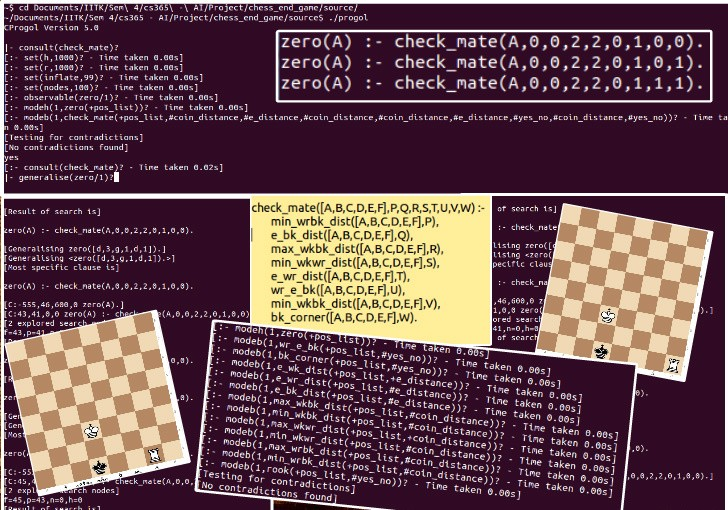
\includegraphics[width=0.8\linewidth]{1.jpg}
\caption{ Check mate (krk) configurations solved fig:ref - http://en.lichess.org/editor}
\end{figure}

\end{block}

%----------------------------------------------------------------------------------------
%	CONCLUSION
%----------------------------------------------------------------------------------------

\begin{block}{Conclusion}

\begin{itemize}
\item The rules obtained for check-mate condition is very intuitive. It can easily be understood and contemplated by humans. Do refer results column. 
\end{itemize}

\end{block}

%----------------------------------------------------------------------------------------
%	REFERENCES
%----------------------------------------------------------------------------------------

\begin{block}{References}
        
\nocite{*} % Insert publications even if they are not cited in the poster
\small{\bibliographystyle{unsrt}
\bibliography{sample}}

\end{block}

%----------------------------------------------------------------------------------------
%	ACKNOWLEDGEMENTS
%----------------------------------------------------------------------------------------

\begin{block}{Acknowledgments}

I thank my senior Mr. Ashudeep Singh and Prof. Amitabha Mukherjee for helping me through this project. 

\end{block}

%----------------------------------------------------------------------------------------
%	CONTACT INFORMATION
%----------------------------------------------------------------------------------------

\setbeamercolor{block title}{fg=black,bg=orange!70} % Change the block title color

\begin{block}{Contact Information}

\begin{itemize}
\item Email: \href{mailto:arunothi@iitk.ac.in}{arunothi@iitk.ac.in}
\item Roll No: 13378
\end{itemize}

\end{block}

%----------------------------------------------------------------------------------------

\end{column} % End of the second column

\begin{column}{.015\textwidth}\end{column} % Empty spacer column

\end{columns} % End of all the columns in the poster

\end{frame} % End of the enclosing frame

\end{document}